\documentclass[../thesis.tex]{subfiles}

\begin{document}

\chapter{Methodology}
\label{chap:method}

\noindent In this chapter we present the methodology and research structure used in this thesis. Some pre-processing of data including imputation and dimensional reduction will also be explained and presented. The implementation of the ML algorithms that produce the results presented in chapter (\ref{chap:exp}).

\section{Overview}

\noindent As stated in the chapter (\ref{chap:intro}), the aim of the thesis is split into two parts. The first part being that of seeing how well various clustering methods perform in producing phenotypically distinct clinical patient groups with HFpEF and HFmrEF? We frame the SL problem in the setting of unsupervised learning and accordingly use the following clustering methods: hierarchical clustering, expectation-maximization and latent class analysis to evaluate which produce the most clinically useful patient groups. The use of these clustering methods are common in the literature (see section \ref{subsec:unsupervisedlearn}) and serves as the main motivation for including them in our analysis. The second part of the problem statement looks at evaluating the accuracy of various classification algorithms in predicting the mortality and re-admission of patients with HFpEF and HFmrEF? In accordance with the literature as presented in section (\ref{sec:predclincout}), we reduce the SL problem of predicting the mortality and re-admission into a two class classification problem where both classes of outcomes are whether or not mortality/re-admission  
\begin{figure}

\centering

\tikzset{every picture/.style={line width=0.75pt}} %set default line width to 0.75pt        

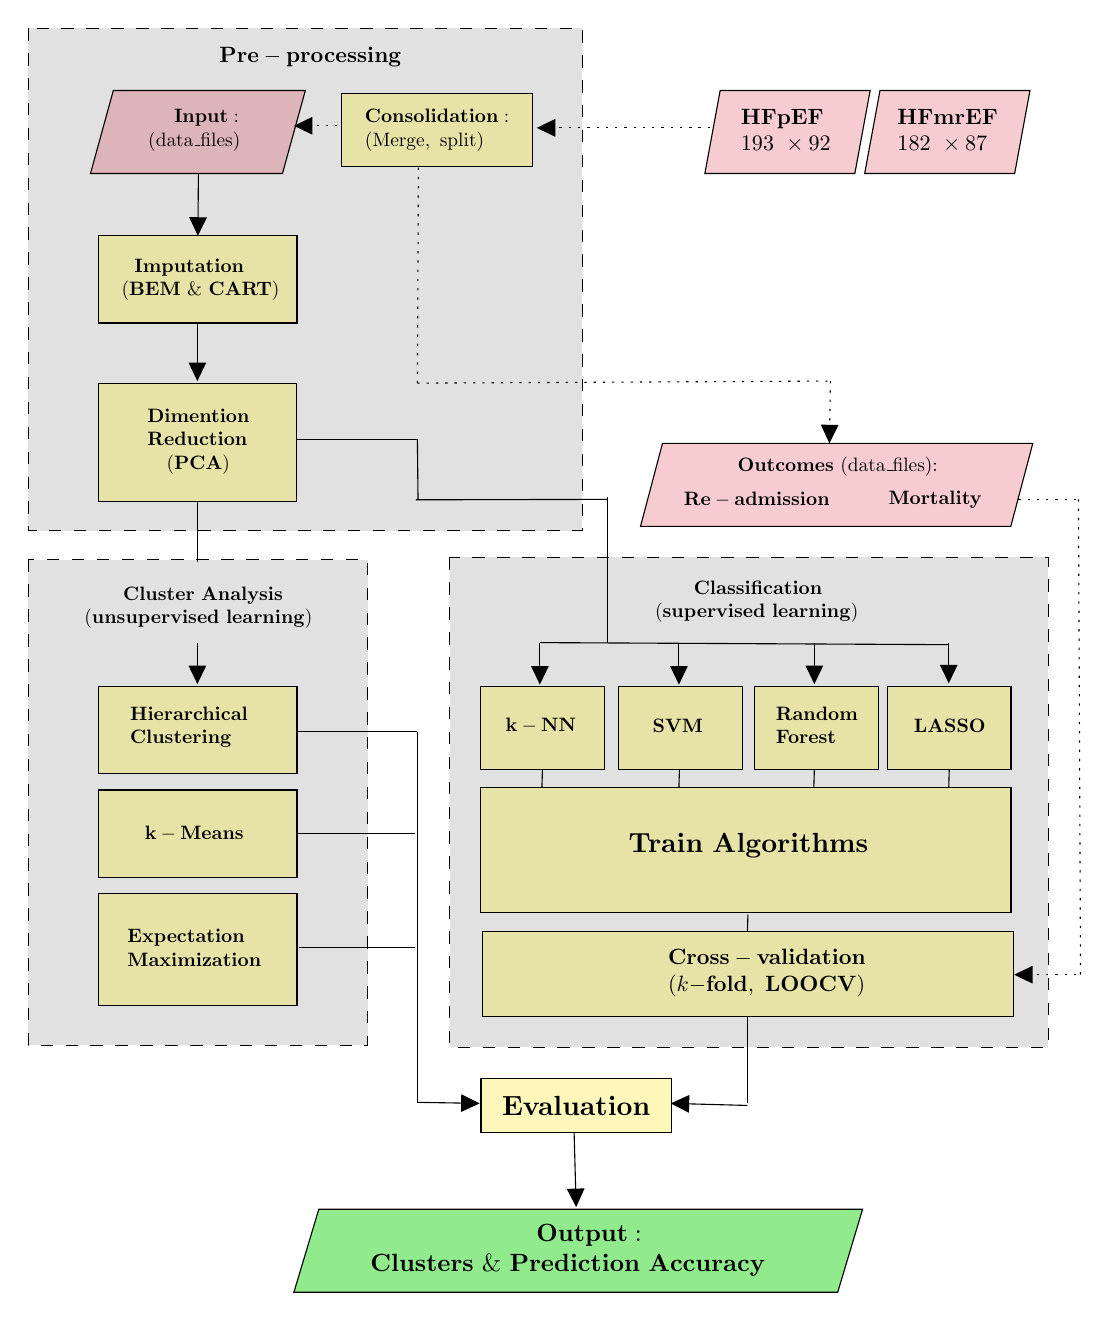
\begin{tikzpicture}[x=0.75pt,y=0.75pt,yscale=-1,xscale=1]
%uncomment if require: \path (0,626); %set diagram left start at 0, and has height of 626

\draw  [fill={rgb, 255:red, 155; green, 155; blue, 155 }  ,fill opacity=0.3 ][dash pattern={on 4.5pt off 4.5pt}]  (2, 5) rectangle (269, 247)   ;
\draw  [fill={rgb, 255:red, 155; green, 155; blue, 155 }  ,fill opacity=0.3 ][dash pattern={on 4.5pt off 4.5pt}]  (205, 260) rectangle (493.5, 496)   ;
\draw  [fill={rgb, 255:red, 155; green, 155; blue, 155 }  ,fill opacity=0.3 ][dash pattern={on 4.5pt off 4.5pt}]  (2, 261) rectangle (165.5, 495)   ;
\draw    (84,75) -- (83.77,103) ;
\draw [shift={(83.75,105)}, rotate = 270.48] [fill={rgb, 255:red, 0; green, 0; blue, 0 }  ][line width=0.75]  [draw opacity=0] (8.93,-4.29) -- (0,0) -- (8.93,4.29) -- cycle    ;

\draw    (83.5,147) -- (83.5,173) ;
\draw [shift={(83.5,175)}, rotate = 270] [fill={rgb, 255:red, 0; green, 0; blue, 0 }  ][line width=0.75]  [draw opacity=0] (8.93,-4.29) -- (0,0) -- (8.93,4.29) -- cycle    ;

\draw    (189.5,344) -- (189.5,523) ;


\draw    (189.5,522.5) -- (217.5,522.97) ;
\draw [shift={(219.5,523)}, rotate = 180.95] [fill={rgb, 255:red, 0; green, 0; blue, 0 }  ][line width=0.75]  [draw opacity=0] (8.93,-4.29) -- (0,0) -- (8.93,4.29) -- cycle    ;

\draw    (248.5,301) -- (248.5,319.22) ;
\draw [shift={(248.5,321.22)}, rotate = 270] [fill={rgb, 255:red, 0; green, 0; blue, 0 }  ][line width=0.75]  [draw opacity=0] (8.93,-4.29) -- (0,0) -- (8.93,4.29) -- cycle    ;

\draw    (315.5,301) -- (315.5,319.22) ;
\draw [shift={(315.5,321.22)}, rotate = 270] [fill={rgb, 255:red, 0; green, 0; blue, 0 }  ][line width=0.75]  [draw opacity=0] (8.93,-4.29) -- (0,0) -- (8.93,4.29) -- cycle    ;

\draw    (380.75,301) -- (380.75,319) ;
\draw [shift={(380.75,321)}, rotate = 270] [fill={rgb, 255:red, 0; green, 0; blue, 0 }  ][line width=0.75]  [draw opacity=0] (8.93,-4.29) -- (0,0) -- (8.93,4.29) -- cycle    ;

\draw    (445.5,301.39) -- (445.5,318.61) ;
\draw [shift={(445.5,320.61)}, rotate = 270] [fill={rgb, 255:red, 0; green, 0; blue, 0 }  ][line width=0.75]  [draw opacity=0] (8.93,-4.29) -- (0,0) -- (8.93,4.29) -- cycle    ;

\draw    (248.5,301) -- (445.5,302) ;


\draw    (348.5,481) -- (348.5,523) ;


\draw    (313.5,523.05) -- (348.5,524) ;

\draw [shift={(311.5,523)}, rotate = 1.55] [fill={rgb, 255:red, 0; green, 0; blue, 0 }  ][line width=0.75]  [draw opacity=0] (8.93,-4.29) -- (0,0) -- (8.93,4.29) -- cycle    ;
\draw  [fill={rgb, 255:red, 248; green, 231; blue, 28 }  ,fill opacity=0.3 ]  (220, 371) rectangle (475.5, 431)   ;
\draw    (281,231) -- (281,301) ;


\draw  [dash pattern={on 0.84pt off 2.51pt}]  (479,232) -- (508,232) ;


\draw  [dash pattern={on 0.84pt off 2.51pt}]  (508,232) -- (509,461) ;


\draw  [dash pattern={on 0.84pt off 2.51pt}]  (479,461) -- (509,461) ;

\draw [shift={(477,461)}, rotate = 0] [fill={rgb, 255:red, 0; green, 0; blue, 0 }  ][line width=0.75]  [draw opacity=0] (8.93,-4.29) -- (0,0) -- (8.93,4.29) -- cycle    ;
\draw  [fill={rgb, 255:red, 248; green, 231; blue, 28 }  ,fill opacity=0.3 ]  (36, 105) rectangle (131.5, 147)   ;
\draw  [fill={rgb, 255:red, 248; green, 231; blue, 28 }  ,fill opacity=0.3 ]  (35.75, 176) rectangle (131.25, 233)   ;
\draw  [fill={rgb, 255:red, 248; green, 231; blue, 28 }  ,fill opacity=0.3 ]  (36, 322) rectangle (131.5, 364)   ;
\draw  [fill={rgb, 255:red, 248; green, 231; blue, 28 }  ,fill opacity=0.3 ]  (36, 372) rectangle (131.5, 414)   ;
\draw  [fill={rgb, 255:red, 248; green, 231; blue, 28 }  ,fill opacity=0.3 ]  (36, 422) rectangle (131.5, 476)   ;
\draw    (131.5,344) -- (189.5,344) ;


\draw    (131.5,393) -- (188.5,393) ;


\draw    (132.5,448) -- (188.5,448) ;


\draw    (188.8,232.2) -- (281,232) ;


\draw    (189.5,203) -- (189.8,232.2) ;


\draw    (131.5,203) -- (189.5,203) ;


\draw  [fill={rgb, 255:red, 248; green, 231; blue, 28 }  ,fill opacity=0.3 ]  (220, 322) rectangle (279.5, 362)   ;
\draw  [fill={rgb, 255:red, 248; green, 231; blue, 28 }  ,fill opacity=0.3 ]  (286.5, 322) rectangle (346, 362)   ;
\draw  [fill={rgb, 255:red, 248; green, 231; blue, 28 }  ,fill opacity=0.3 ]  (352, 322) rectangle (411.5, 362)   ;
\draw  [fill={rgb, 255:red, 248; green, 231; blue, 28 }  ,fill opacity=0.3 ]  (416, 322) rectangle (475.5, 362)   ;
\draw    (249.5,371) -- (249.75,362) ;


\draw    (315.5,371) -- (315.75,362) ;


\draw    (380.5,371) -- (380.75,362) ;


\draw    (445.5,371) -- (445.75,362) ;


\draw  [fill={rgb, 255:red, 248; green, 231; blue, 28 }  ,fill opacity=0.3 ]  (221, 440) rectangle (476.5, 481)   ;
\draw    (83.5,233) -- (83.5,262) ;


\draw    (348.5,440) -- (348.75,432) ;


\draw    (265,537) -- (265.94,571) ;
\draw [shift={(266,573)}, rotate = 268.40999999999997] [fill={rgb, 255:red, 0; green, 0; blue, 0 }  ][line width=0.75]  [draw opacity=0] (8.93,-4.29) -- (0,0) -- (8.93,4.29) -- cycle    ;

\draw  [fill={rgb, 255:red, 208; green, 2; blue, 27 }  ,fill opacity=0.2 ] (335.38,35) -- (407.64,35) -- (400.26,75) -- (328,75) -- cycle ;
\draw    (83.5,301) -- (83.5,319) ;
\draw [shift={(83.5,321)}, rotate = 270] [fill={rgb, 255:red, 0; green, 0; blue, 0 }  ][line width=0.75]  [draw opacity=0] (8.93,-4.29) -- (0,0) -- (8.93,4.29) -- cycle    ;

\draw  [dash pattern={on 0.84pt off 2.51pt}]  (189.5,176) -- (388.5,175) ;


\draw  [dash pattern={on 0.84pt off 2.51pt}]  (388.5,175) -- (388.03,203) ;
\draw [shift={(388,205)}, rotate = 270.95] [fill={rgb, 255:red, 0; green, 0; blue, 0 }  ][line width=0.75]  [draw opacity=0] (8.93,-4.29) -- (0,0) -- (8.93,4.29) -- cycle    ;

\draw  [dash pattern={on 0.84pt off 2.51pt}]  (189.5,176) -- (190,72) ;


\draw  [dash pattern={on 0.84pt off 2.51pt}]  (132,52) -- (152,52) ;

\draw [shift={(130,52)}, rotate = 0] [fill={rgb, 255:red, 0; green, 0; blue, 0 }  ][line width=0.75]  [draw opacity=0] (8.93,-4.29) -- (0,0) -- (8.93,4.29) -- cycle    ;
\draw  [dash pattern={on 0.84pt off 2.51pt}]  (249,53) -- (331,53) ;

\draw [shift={(247,53)}, rotate = 0] [fill={rgb, 255:red, 0; green, 0; blue, 0 }  ][line width=0.75]  [draw opacity=0] (8.93,-4.29) -- (0,0) -- (8.93,4.29) -- cycle    ;
\draw  [fill={rgb, 255:red, 208; green, 2; blue, 27 }  ,fill opacity=0.2 ] (43,35) -- (135.5,35) -- (124.5,75) -- (32,75) -- cycle ;
\draw  [fill={rgb, 255:red, 139; green, 233; blue, 134 }  ,fill opacity=0.95 ] (142,574) -- (404,574) -- (392,614) -- (130,614) -- cycle ;
\draw  [fill={rgb, 255:red, 208; green, 2; blue, 27 }  ,fill opacity=0.2 ] (307.6,205) -- (486,205) -- (475.4,245) -- (297,245) -- cycle ;
\draw  [fill={rgb, 255:red, 208; green, 2; blue, 27 }  ,fill opacity=0.2 ] (412.38,35) -- (484.64,35) -- (477.26,75) -- (405,75) -- cycle ;

\draw (82,54) node [scale=0.7]  {$ \begin{array}{l}
\ \ \ \ \mathbf{Input:}\\
(\mathrm{data\_files})
\end{array}$};
\draw (85,126) node [scale=0.7]  {$ \begin{array}{l}
\ \ \mathbf{Imputation}\\
\mathbf{( BEM\ \&\ CART)}
\end{array}$};
\draw (84,204) node [scale=0.7]  {$ \begin{array}{l}
\mathbf{Dimention}\\
\mathbf{Reduction}\\
\ \ \ \mathbf{( PCA)}
\end{array}$};
\draw (81,342) node [scale=0.7]  {$ \begin{array}{l}
\mathbf{Hierarchical\ }\\
\mathbf{Clustering}
\end{array}$};
\draw (82,393) node [scale=0.7]  {$\mathbf{k-Means}$};
\draw (82,449) node [scale=0.7]  {$ \begin{array}{l}
\mathbf{Expectation}\\
\mathbf{Maximization}
\end{array}$};
\draw (84,284) node [scale=0.7]  {$ \begin{array}{l}
\ \ \ \ \ \ \mathbf{Cluster\ Analysis}\\
\mathbf{( unsupervised\ learning)}
\end{array}$};
\draw  [fill={rgb, 255:red, 248; green, 231; blue, 28 }  ,fill opacity=0.3 ]   (220.16, 511) rectangle (311.84, 537)   ;
\draw (266,524) node   {$\mathbf{Evaluation}$};
\draw (249,341) node [scale=0.7]  {$\mathbf{k-NN}$};
\draw (315,341) node [scale=0.7]  {$\mathbf{SVM}$};
\draw (382,342) node [scale=0.7]  {$ \begin{array}{l}
\mathbf{Random}\\
\mathbf{Forest}
\end{array}$};
\draw (446,341) node [scale=0.7]  {$\mathbf{LASSO}$};
\draw (349,460) node [scale=0.8]  {$ \begin{array}{l}
\ \ \ \ \ \mathbf{Cross-validation}\\
\ \ \ \ \ \mathbf{(} k\mathbf{-fold} ,\ \mathbf{LOOCV)}
\end{array}$};
\draw (353,281) node [scale=0.7]  {$ \begin{array}{l}
\ \ \ \ \ \ \mathbf{Classification}\\
\mathbf{( supervised\ learning)}
\end{array}$};
\draw (349,399) node   {$\mathbf{Train\ Algorithms}$};
\draw (262,594) node [scale=0.9]  {$ \begin{array}{l}
\ \ \ \ \ \ \ \ \ \ \ \ \ \ \ \ \ \ \ \ \mathbf{Output:}\\
\mathbf{Clusters\ \&\ Prediction\ Accuracy}
\end{array}$};
\draw (353,232) node [scale=0.7]  {$\mathbf{Re-admission}$};
\draw (439,232) node [scale=0.7]  {$\mathbf{Mortality}$};
\draw (392,216) node [scale=0.7]  {$\mathbf{Outcomes\ (}\mathrm{data\_files})\mathbf{:}$};
\draw (445,55) node [scale=0.8]  {$ \begin{array}{l}
\mathbf{HFmrEF}\\
182\ \times 87
\end{array}$};
\draw (367,55) node [scale=0.8]  {$ \begin{array}{l}
\mathbf{HFpEF}\\
193\ \times 92
\end{array}$};
\draw  [fill={rgb, 255:red, 248; green, 231; blue, 28 }  ,fill opacity=0.3 ]   (153.05, 36.5) rectangle (244.95, 71.5)   ;
\draw (199,54) node [scale=0.7]  {$ \begin{array}{l}
\mathbf{Consolidation} :\\
(\mathrm{Merge,\ split})
\end{array}$};
\draw (138,19) node [scale=0.8]  {$\mathbf{Pre-processing}$};

\end{tikzpicture}


\caption[Machine learning procedure adopted in the thesis]{\textit{Machine learning procedure adopted in the thesis}}
\label{fig:ML_proc_thesis}
\normalsize
\end{figure}\noindent occurred. The classification methods that we will be evaluating are: k-nearest neighbours (k-NN), support vector machines (SVM), random forest and least absolute shrinkage and selection operator (LASSO) algorithms. All the algorithms are much used in the literature. The motivation behind the use of the chosen algorithms has always been to confirm with the practices done in the literature. We do however need to emphasize that many algorithms exists that can be used to further broaden the analysis done in this thesis. This is something we have not done due to limitations.\\
\indent The machine learning procedure adopted in this thesis is illustrated in figure (\ref{fig:ML_proc_thesis}). The structure starts by pre-processing the data. This includes imputation of missing data to ensure that the data is balanced and dimensional reduction to address eventual problems with higher dimensional multi-correlated variables. Both the pre-processing steps are explained in further detail later in this chapter (see section \ref{sec:data}). After the pre-processing is done the structure continues by first addressing the cluster analysis. Being that the dimension reduction is relevant for both the cluster analysis and classification. We use the components derived from the dimension reduction process as input into both the clustering and classification algorithms evaluated. The cluster analysis runs the produced components through the three cluster algorithms (hierarchical clustering, expectation maximization and latent component analysis). After the procedure is done, three sets of clusters are produced and the next step is to evaluate the clusters to assess their medical usefulness. The supervised classification track on the other hand is structured in a somewhat different way. First the procedure starts by removing the labels of the various clinical outcomes associated with the given patients. After this is done the chosen components from the dimension reduction is run through the four classification algorithms (k-NN, SVM, RF and LASSO) and the data is trained and validated to produce approximately unbiased estimates of the test errors/accuracy. After the data is run thought the classification process and the accuracy are produced, the algorithms are ranked and evaluated accordingly. The outputs of the whole ML procedure are i) clinical clusters with (maybe) distinct phenotypical properties and ii) the accuracy of the various classification algorithms in predicting re-admission and mortality in the data sets.\\
\indent All the processes mentioned in the ML procedure in figure (\ref{fig:ML_proc_thesis}) are developed using the \texttt{R} statistical programming language (version 3.4.4 - \textit{Someone to Lean On}) \citep{Rsoftware2018} with RStudio as the integrated development environment (IDE), version 1.1.423 \citep{RStudio2018}. We use a number of external libraries and self-made algorithms in order to make the process more efficient. Data description with variable explanations, descriptive statistics and some relevant plot can be fount in appendix (\ref{chap:data_desc}). The source code used to produce all the results in this thesis can be found in appendix (\ref{chap:souce_code}). As we now have given an overview of the ML procedure used in this thesis we move on to presenting the data.

\section{Data}
\label{sec:data}

\noindent The data used is comprised of two data sets (\texttt{data\_use\_HFpEF.mat}, $N = 182$ and \texttt{data\_use\_HFmrEF.mat}, $N = 193$). The data was collected by the medical staff at a tertiary hospital in the United Kingdom. At this particular hospital NT-proBNP led heart failure service were run on all patients with suspected heart failure. All patients with suspected HF based on an assessment of the HF probability and raised NT-proBNP/BNP levels (see figure \ref{fig:esc_algo_hf}) were included and forwarded for an echocardiography. An expert HF physician reviewed all the patients after the echocardiography was performed. The patients were diagnosed with HF according to the 2016 ESC guidelines \citep{ponikowski2016}. Accordingly, signs and symptoms of HF, raised NP values, echocardiographic results including left ventricular ejection fraction (LVEF) and evidence of structural or functional heart abnormalities were the primary basis for the assessment done by the hospitals cardiac physicians. After the diagnosis patients were categorized based on LVEF following the ESC guidelines, i.e. patients with LVEF $>$ 50\% were classified as HFpEF and those with $40 \leq$ LVEF $< 50$ as HFmrEF. The patients with LVEF $<$ 40\%, greater than moderate valvular heart disease and prior cardiac transplantation were excluded. The data was collected over a one year period from October 10th, 2014 to October 9th, 2015. In total 375 patients were analyzed over this one year period with data from 126 clinical features being recorded. The outcomes were evaluated through the hospitals databases and mortality was confirmed with the Office for National Statistics. All the data was collected as part of the hospitals approved Clinical Audit.\\
\indent As mentioned in the previous section, we reduced the SL problem in the supervised learning part of the ML procedure to that of a two class classification problem. The way in which this was done was with respect to the various \texttt{patient\_groups} in the data. The patients were grouped based on various outcomes. In total six outcome categories were defined in the data sets. The outcome categories are as follows: \texttt{IN} - inhospital death, \texttt{Z} -



\begin{footnotesize}
\begin{tabularx}{\textwidth}{p{0.8cm}LLLLp{0.8cm}LLLL}
\caption{Clinical outcome classes}\label{tab:outcomes_class}\\
\toprule
\multicolumn{4}{c}{HFpEF} & \multicolumn{4}{c}{HFmrEF}\\
\midrule
\textbf{Group} & Dead? & Readm? & $n$ & \% Tot & \textbf{Group} & Dead? & Readm? & $n$ & \% Tot \\ 
\midrule
\endfirsthead
\caption*{\textbf{Table \ref{tab:outcomes_class}:} Clinical outcome classes (\textit{continued})}\\
\toprule
\multicolumn{4}{c}{HFpEF} & \multicolumn{4}{c}{HFmrEF}\\
\midrule
\textbf{Group} & Dead? & Readm? & $n$ & \% Tot & \textbf{Group} & Dead? & Readm? & $n$ & \% Tot \\ 
\midrule
\endhead
R & no & no & 85 & 0.440 & R & no & no & 101 & 0.555 \\ 
U & no & yes & 40 & 0.207 & U & no & yes & 19 & 0.104 \\ 
X, R & yes & no & 29 & 0.150 & Y & yes & no & 15 & 0.082 \\ 
V & no & yes & 10 & 0.052 & IN & yes & no & 8 & 0.044 \\ 
IN & yes & no & 7 & 0.036 & X & yes & no & 8 & 0.044 \\ 
Y, U & yes & yes & 7 & 0.036 & Z & yes & no & 7 & 0.038 \\ 
Y, V & yes & yes & 7 & 0.036 & Y, U & yes & yes & 6 & 0.033 \\ 
X, U & yes & yes & 6 & 0.031 & V & no & yes & 5 & 0.027 \\ 
X & yes & no & 1 & 0.005 & X, U & yes & yes & 5 & 0.027 \\ 
Y & yes & no & 1 & 0.005 & Y, V & yes & yes & 4 & 0.022 \\ 
&  &  &  &  & X, V & yes & yes & 3 & 0.016 \\ 
&  &  &  &  & Z, V & yes & yes & 1 & 0.005 \\
\midrule
\end{tabularx}
\end{footnotesize}

\noindent dead within 30 days, \texttt{Y} - dead within 1 year, \texttt{X} - dead by Fluorouracil (medication), \texttt{V} - cardiac readmission within 30 days, \texttt{U} - readmission and \texttt{R} - the rest. The various combinations of the outcome classes found in the data sets and the way in which they were classified are listed in table (\ref{tab:outcomes_class}). From this table we can see that approximately 36\% of all the patients in the HFpEF data set were readmitted in some form, i.e either within 30 days or more. In the HFmrEF data set this number was somewhat smaller being approximately 23\%. The number also differed with respect to the whether the patients were confirmed deceased or not. In the HFpEF data set approximately 30\% of the patients were confirmed deceased and in the HFmrEF data set this number was 31\%. Further descriptive statistics on the data can be found in appendix (\ref{sec:desc_stat}). The source code for the two-class outcome classification shown in table (\ref{tab:outcomes_class}) can be found in appendix (\ref{sec:app_desc_stat}).\\
\indent As the data used in this thesis is cross-sectional, we need to emphasize that it is not perfect. Limitations to the data sets are many and one of the most primary of them is in regard to missing data.


\subsection{Missing Data}
\label{subsec:miss_data}

\noindent Missing values in data is a very important concept in data management and a highly prevalent problem in any data analysis. If one does not handle missing values properly this may lead to inaccurate or invalid inference being drawn from the data. Results where improper treatment of missing data is present may differ significantly from those where missing data is not present. In medical research it is not uncommon for data about a given patient to be missing. One typically considered missing data from patients clinical variables as being the values that are not directly observed \citep{ibrahim2012missing}. Data can be missing due to a number of reasons. In clinical research some reasons may include: poor communication with study subject, difficulties assessing the clinical outcomes, 
lack of consolidation from test, duration of trial etc. The latter is often a reason for missing data as longer trials tend to produce more risk of missing data. Especially considering that patients often run the risk of being dropped from the study before completion \citep{myers2000handling}.\\
\indent In our data sets the problem with missing values is very present. In the HFpEF data set a total of 2383 observations, i.e. approximately 13.3\% of the data set is missing. In the non-indicator variables, the largest contributors to this can be attributed to the lack of glucose measured (\texttt{glucose}, 5.7\%), failure to register time to HF admission (\texttt{timetohfadm}, 5.2\%), ferritin levels (\texttt{ferritin}, 5.1\%), lateral peak velocity of systolic pulmonary vein flow (\texttt{laterals}, 5.0\%), glycohemoglobin (\texttt{hba1c}, 4.7\%) and transferrin saturation (\texttt{tsat}, 4.2\%). These variables contribute to approximately 29.9\% of the total 



\begin{footnotesize}
\begin{tabularx}{\textwidth}{P{2.3cm}LLLLP{2.7cm}LLLL}
\caption{Summary of missing values}\label{tab:top_missing}\\
\toprule
\multicolumn{5}{c}{HFpEF} & \multicolumn{5}{c}{HFmrEF}\\
\midrule
\textbf{Variable (V)}& \#Na & \%$n$ & \%Na & \%V & \textbf{Variable (V)} & \#Na & \%$n$ & \%Na & \%V \\ 
\midrule
\endfirsthead
\caption*{\textbf{Table \ref{tab:top_missing}:} Summary of missing values (\textit{Continued})}\\
\toprule
\multicolumn{5}{c}{HFpEF} & \multicolumn{5}{c}{HFmrEF}\\
\midrule
\textbf{Variable (V)}& \#Na & \%$n$ & \%Na & \%V & \textbf{Variable (V)} & \#Na & \%$n$ & \%Na & \%V \\ 
\midrule
\endhead
grand.tot & 973 & 0.092 & 1 &  & grand.tot & 2108 & 0.211 & 1 &  \\ 
\midrule
irondef & 124 & 0.012 & 0.127 & 0.642 & bmiadmission & 178 & 0.018 & 0.084 & 0.978 \\ 
timetohfadm & 124 & 0.012 & 0.127 & 0.642 & admissionwgt & 131 & 0.013 & 0.062 & 0.720 \\ 
ferritin & 122 & 0.011 & 0.125 & 0.632 & irondef & 130 & 0.013 & 0.062 & 0.714 \\ 
tsat & 99 & 0.009 & 0.102 & 0.513 & obesity & 129 & 0.013 & 0.061 & 0.709 \\ 
ironlevels & 98 & 0.009 & 0.101 & 0.508 & ferritin & 128 & 0.013 & 0.061 & 0.703 \\ 
pasp & 71 & 0.007 & 0.073 & 0.368 & breathless & 127 & 0.013 & 0.06 & 0.698 \\ 
bmiadmission & 45 & 0.004 & 0.046 & 0.233 & ironlevels & 112 & 0.011 & 0.053 & 0.615 \\ 
ee & 41 & 0.004 & 0.042 & 0.212 & tsat & 111 & 0.011 & 0.053 & 0.610 \\ 
ecgqrsduration & 36 & 0.003 & 0.037 & 0.187 & pasp & 110 & 0.011 & 0.052 & 0.604 \\ 
ecgrate & 34 & 0.003 & 0.035 & 0.176 & ecgqrsduration & 105 & 0.01 & 0.05 & 0.577 \\
\midrule
\end{tabularx}
\end{footnotesize}
\newpage
\noindent missing values. In the HFmrEF data set, the picure is very much different. In general we can say that this data set has a much larger presence of missing values. In total 3586 observations, i.e. approximately 22.4\% of the data is missing. The largest non-indicator contributors are: inability to record the body mass index (BMI) at admission (\texttt{bmiadmission}, 5\%), the weight after patients are discharged (\texttt{dischargeweight}, 4.9\%), measures of troponin (\texttt{troponin}, 3.9\%), the time to first cardiac hospitalization (\texttt{timetofirstcardiachospitalisation}, 3.9\%) and the patients weight at admission (\texttt{admissionwgt}, 3.7\%).


\subsection{Imputation}
\label{subsec:impu}

\subsection{Dimensional Reduction}
\label{subsec:dim_red}

\section{Clustering Patient Groups}
\label{sec:cluster_pat_gro}

\subsection{Hierarchical}
\label{subsec:hierarchical}

\subsection{Expectation-Maximization}
\label{subsec:em}

\subsection{Latent Class Analysis}
\label{subsec:lca}

\section{Classifying Clinical Outcomes}
\label{sec:classify_clin_out}

\subsection{k-Nearest Neighbours (k-NN)}
\label{subsec:knn}

\subsection{Support Vector Machines (SVM)}
\label{subsec:svm}

\subsection{Random Forrest}
\label{subsec:random_forr}

\subsection{LASSO}
\label{subsec:lasso}

\section{Validation}
\label{sec:validation}

\subsection{k-Fold}
\label{subsec:k_fold}

\subsection{Leave One Out}
\label{subsec:loocv}

\end{document}